\section{Outils mathématiques utilisés dans la reconstruction d'images ct par le compressed sensing}
\subsection{Famille de méthodes de reconstruction}
% [Speech] La reconstruction tomographique repose sur un problème inverse : retrouver l’image à partir de ses projections ou son sinogramme
\begin{frame}{Famille de méthodes de reconstruction}
    \only<1>{
        % [Speech] Permet de determiner le coefficient d'attenuation
        \begin{columns}
            \column{0.5\textwidth}
            \begin{block}{Loi de Beer-Lambert} 
                \begin{equation}
                    I(x) = I_0 e^{-A(x)\, x}
                \end{equation}
                où \begin{itemize}
                    \item $x$ est la distance parcourue par le rayon $X$
                    \item $I(x)$ est l'intensité final 
                    \item $I_0$ est l'intensité initiale
                    \item $A(x)$ est la proportion de photons absorbés sur un distance $x$
                \end{itemize}
            \end{block}

            \column{0.5\textwidth}
            \begin{block}{Sinogramme}
                \begin{equation}
                    ln(I(x0)/I(x1)) = \int_{x0}^{x1} A(x)\, dx
                \end{equation}
                où $ln(I(x0)/I(x1))$ désigne les données de projection, communément appelées le sinogramme
            \end{block}
        \end{columns}
    }
    \only<2>{
        \begin{columns}
            \column{0.33\textwidth}
            \begin{figure}[H]
                \centering
                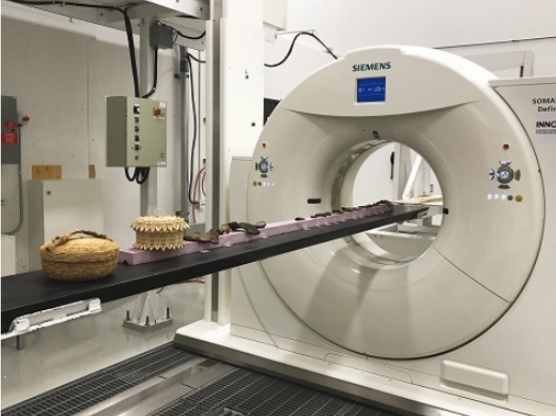
\includegraphics[height=3cm, keepaspectratio]{../images/ct_device.png}
                \caption{Appareil de tomodensitométrie}
                \label{fig :tomography_device}
            \end{figure}

            \column{0.33\textwidth}
            \begin{figure}[H]
                \centering
                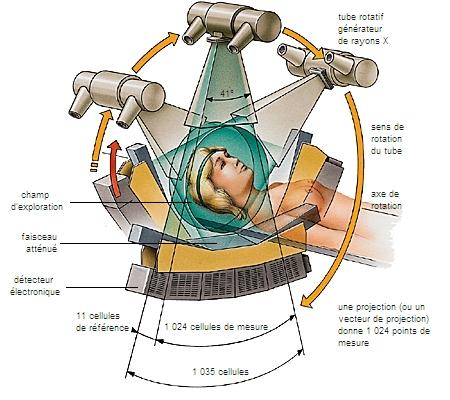
\includegraphics[height=3cm, keepaspectratio]{../images/ct_scan_operation.jpeg}
                \caption{Fonctionnement de la CT-Scan}
                \label{fig :tomography_device_operation}
            \end{figure}

            \column{0.33\textwidth}
            \begin{figure}[H]
                \centering
                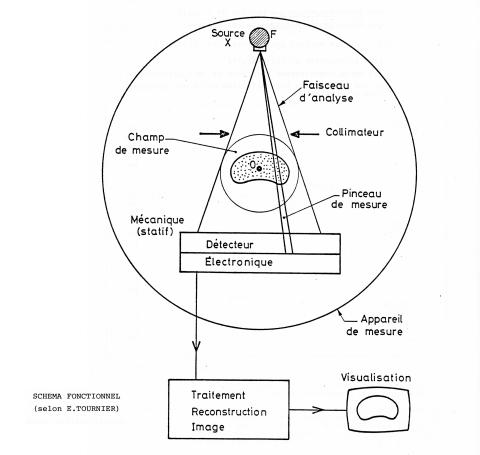
\includegraphics[height=3cm, keepaspectratio]{../images/ct_scan_reconstruction_process.jpeg}
                \caption{Processus de reconstruction}
                \label{fig :tomography_device_operation}
            \end{figure}
        \end{columns}
    }
    \only<3>{
        \begin{block}{Filter Back Projection (FBP)}
            \begin{equation}
                f(x,y) \approx \frac{1}{2}\,\mathcal{B}\!\left(\mathcal{F}^{-1} S' \star \mathcal{R}f \right)(x,y).
                \label{eq:FBP_varphi_approx}
            \end{equation}
            où \begin{itemize}
                \item $\mathcal{F}^{-1}$ est l'inverse de la transformée de Fourier
                \item $\mathcal{B}$ est la retroprojection
                \item $S'$ est un filtre filtre passe-bas
                \item $\mathcal{R}f$ est la transformée de Radon de $f$
            \end{itemize}
        \end{block}
    }
    \only<4>{
        \begin{block}{Approches discrète}
            \begin{equation}
                g=Af
            \end{equation}
            où \begin{itemize}
                    \item $A$ (matrice système) représente la transformée de Radon discrète
                    \item $g$ est le sinogramme mesuré
                    \item $f$ est l'image à reconstruire
            \end{itemize}
        \end{block}
    }\only<4>{
        % [Speech] Un signal peut être reconstruit à partir de très peu de mesures s'il est parcimonieux dans un domaine de représentation adapté.
        \begin{block}{Compressive Sensing (CS)}
            \begin{equation}
                \min_f ||A f - g||^2 + \lambda \Phi(f)
            \end{equation}
                où $\Phi(f)$ = régularisation (sparsité)

        \end{block}
    }
    \only<5>{
        \begin{figure}[H]
            \centering
            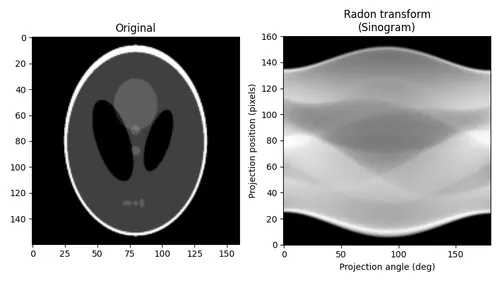
\includegraphics[height=3cm, keepaspectratio]{../images/sinogram_and_reconstructed_image.png}
            \caption{Pair image-sinogramme}
            \label{fig :tomography_device_operation}
        \end{figure}
    }
\end{frame}
